% TODO acronyms
\chapter{The \emph{Weather Importer}}
\label{ch:weather_importer}

In previous chapters, two topics are discussed that are relevant for this chapter: Chapter~\ref{ch:weather_data} digs into the details of weather services that are available via Internet, with the example of the API by the \emph{Norwegian Meteorological Institute} (\yrno) that is found to best fit the requirements found at the \thinkhome project. Chapter~\ref{ch:thinkhomeweather_ontology} describes the design of the \smarthomeweather ontology. Eventually, the ontology needs to be populated with data, i.e. individuals that comprise the current and future state of the weather at the desired location.

For that process, a standalone Java application has been developed. As its main purpose is to import weather data, it was named \emph{Weather Importer}.

At its current state of development, \emph{Weather Importer} obtains data only from \yrno in order to provide a reference implementation being both simple and functional, but it is designed to allow simple integration of other weather services that are available via Internet as well as data from local weather sensors.

The classes are arranged in two packages, \texttt{model} and \texttt{main}. The \texttt{model} package contains an object-oriented data model for the weather data being processed (see section~\ref{sec:importer_model}). All other classes belong to the \texttt{main} package, including the \texttt{Main} class providing the \texttt{main} method, the classes \texttt{TurtleStatement} and \texttt{TurtleStore} for output in \emph{Turtle syntax}\cite{Turtle} (see section~\ref{subsec:importer_turtle}), the interface \texttt{Importer}, and its reference implementation \texttt{YrNoImporter} (see section~\ref{subsec:importer_fetch}), \texttt{WeatherImporterProperties} which encapsulates the \emph{properties file} (see section~\ref{sec:importer_application}), and \texttt{WeatherImporterException}, an exception class that is used throughout the application.

All classes belonging to \emph{Weather Importer} include comments suitable for use with the \emph{Javadoc Tool}~\cite{javadoc}.

\section{The data model}
\label{sec:importer_model}

The core of \emph{Weather Importer} is formed by an object-oriented data model that can be found in the \texttt{model} package. This package contains classes that are to be instantiated in order to encapsulate all data that is collected from weather sensors and services. After processing the data in a manner that makes it suitable for use within the \smarthomeweather ontology, individuals and statements are generated and added to the ontology.

\begin{figure}
\centering
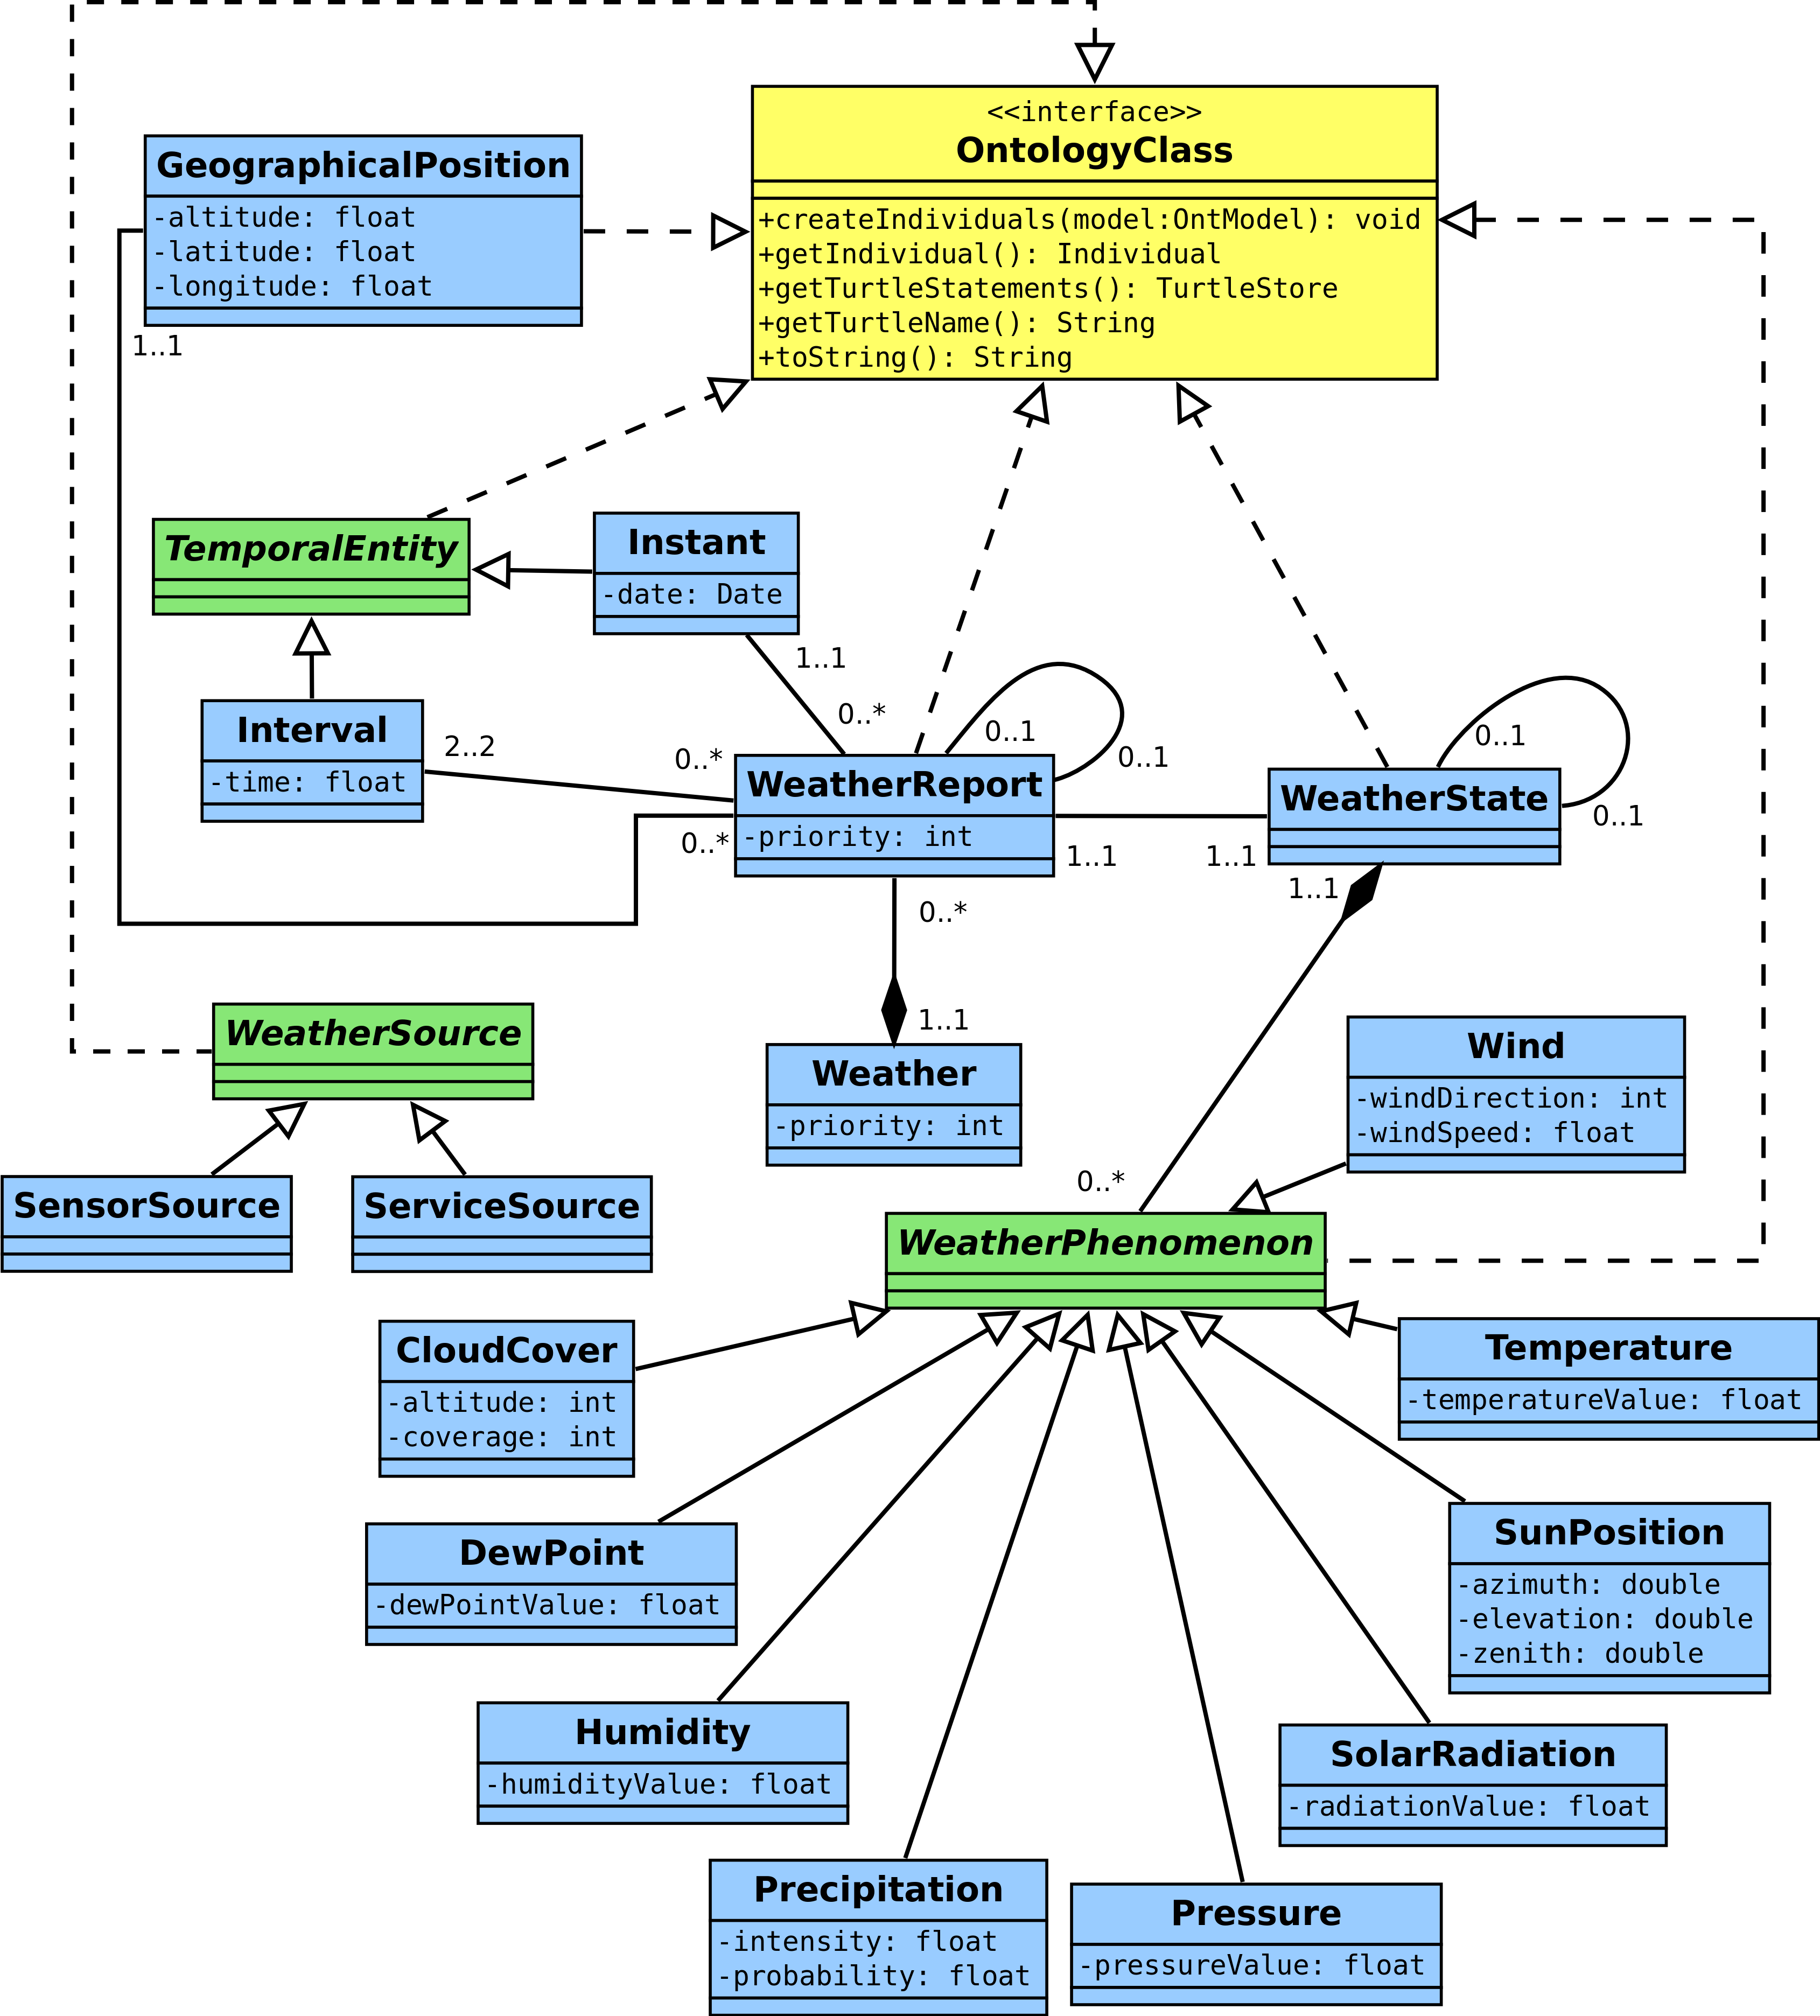
\includegraphics[width=\textwidth]{figures/diagrams/importer-model.pdf}
\caption{The domain model used in \emph{Weather importer}. See figure~\ref{fig:importer_model2} for a simplified diagram that shows only the most important classes.}
\label{fig:importer_model1}
\end{figure}

\begin{figure}
\centering
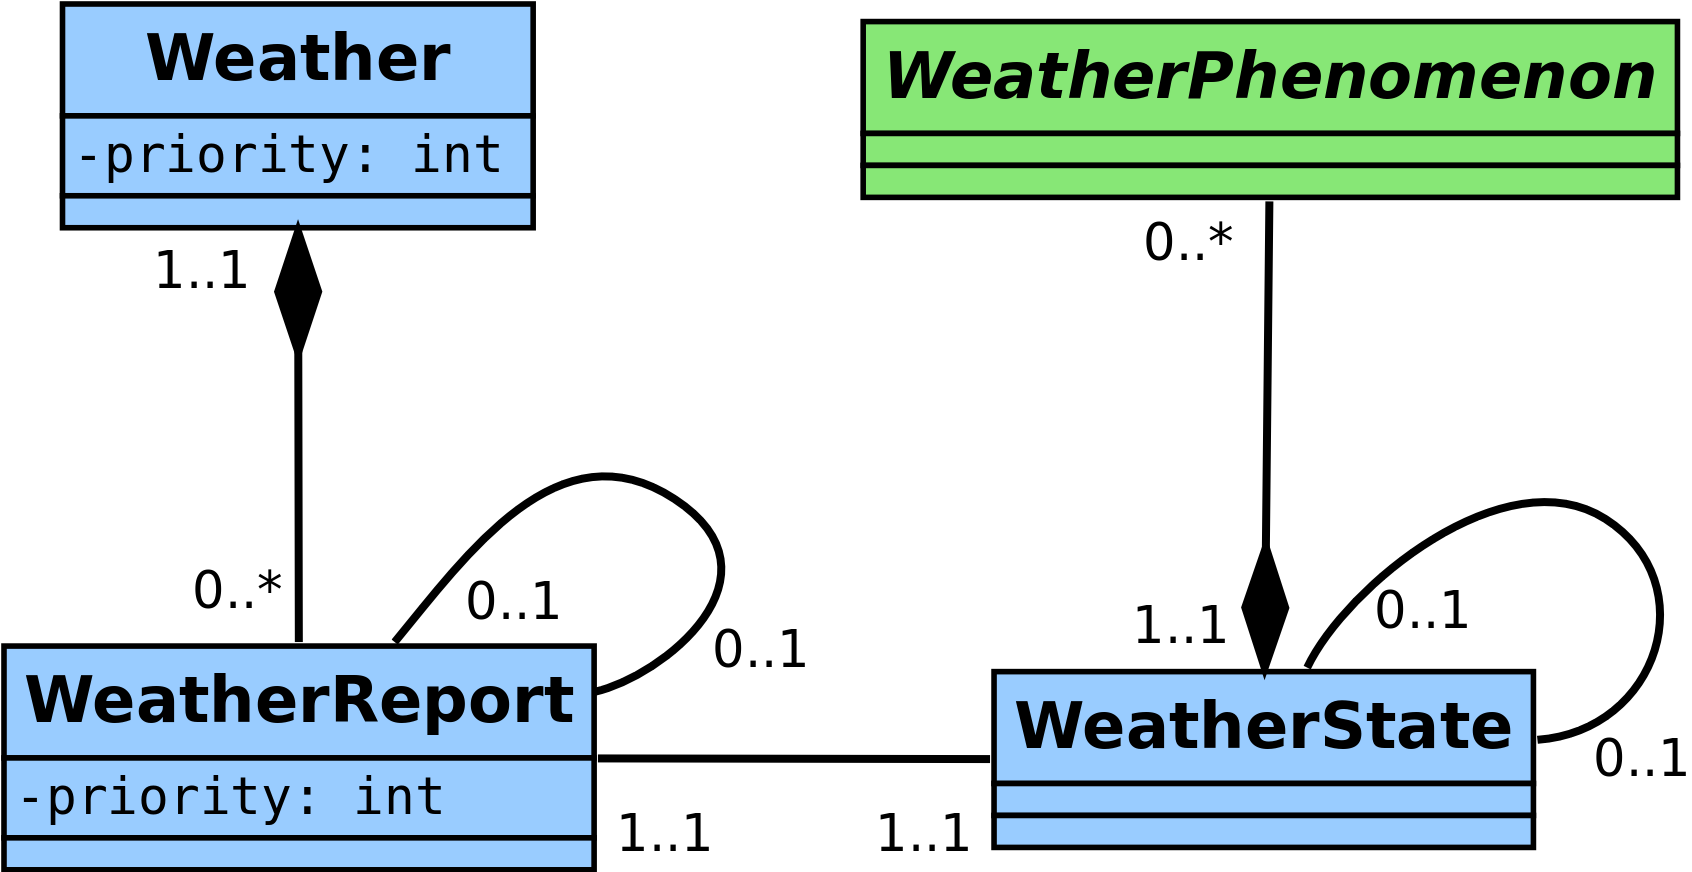
\includegraphics[width=.5\textwidth]{figures/diagrams/importer-model-simple.pdf}
\caption{The most important classes of the domain model used in \emph{Weather importer}. Refer to figure~\ref{fig:importer_model1} for a diagram showing all classes.}
\label{fig:importer_model2}
\end{figure}

The domain model in the package \texttt{model} which resembles the structure of the \smarthomeweather ontology is depicted in the \emph{UML} class diagram in figure~\ref{fig:importer_model1}; to give an overview, figure~\ref{fig:importer_model2} shows a simplified class diagram that shows only the most important classes \texttt{Weather}, \texttt{WeatherReport}, \texttt{WeatherState}, and \texttt{WeatherPhenomenon}.

Other than its name suggests, \texttt{OntologyClass} is an interface that is implemented by every class that corresponds to a concept (class) in the ontology. That interface defines a set of methods which are necessary to export an object's data either to individuals and statements for adding them to the ontology using \emph{Apache Jena}~\cite{apache_jena} or to a representation of the individuals and statements in \emph{Turtle syntax} (see section~\ref{sec:importer_application} below). The methods defined by \texttt{OntologyClass} are:
\begin{itemize}
  \item \texttt{createIndividuals()} creates individuals and statements holding the data that is stored in the object and adds them to the ontology. The method calls \texttt{createIndividuals()} for any objects that are connected to this object, with the exception of instances of \texttt{WeatherState} and \texttt{WeatherReport} that are linked together via the properties \texttt{previousState} and \texttt{previousReport}, respectively.
  
  \item \texttt{getIndividual()} returns the \texttt{Individual} object previously created by the method \texttt{createIndividuals()} that represents the main ontology individual described by the object. In some classes, due to the structure of the \smarthomeweather ontology and the ontologies being imported, calling \texttt{createIndividuals()} will add more than one individual to the ontology, e.g. an \texttt{Instant} creates an individual of type \Egls{instant} and one of type \emph{DateTimeDescription}\footnote{\emph{DateTimeDescription} is defined by \emph{OWL-Time} as the concept that represents the timestamp of an \Egls{instant}; the property \emph{inDateTime} links an instance of \emph{DateTimeDescription} to an instance of \Egls{instant}.}. \texttt{getIndividual()} will return the \texttt{Individual} object representing the \Egls{instant} individual; the corresponding \emph{DateTimeDescription} object can be obtained by querying the ontology for the statement having the previously returned
  \Egls{instant} individual as subject and the property \emph{inDateTime} as predicate.
  
  \item \texttt{getTurtleStatements()} returns an instance of \texttt{TurtleStore} that contains a set of \texttt{TurtleStatement} objects each representing an RDF triple in \texttt{Turtle syntax}. The instance being returned contains all data that calling \texttt{createIndividuals()} would add to the ontology. See section~\ref{subsec:importer_turtle} for details.
  
  \item \texttt{getTurtleName()} returns the qualified name of the individual represented by the object that is used in in the \texttt{TurtleStatement}s returned by calling \texttt{getTurtleStatements()}. In case \texttt{createIndividuals()} creates more than one individual, the method only yields the name of the individual returned by \texttt{getIndividual()}.
  
  \item \texttt{toString()} returns a textual representation of the object (for debugging purposes).
\end{itemize}

The classes inside the package \texttt{model} are:
\begin{itemize}
  \item \texttt{GeographicalPosition} resembles the concept \Egls{point} of the \emph{Basic Geo (WGS84 lat/long) Vocabulary}\cite{wgs84_vocabulary} that is imported into the \smarthomeweather ontology.
  
  \item \texttt{TemporalEntity} corresponds to the concept \Egls{temporal entity} in the \emph{OWL-Time}\cite{owl-time} ontology. The are two sub-classes, \texttt{Instant} and \texttt{Interval} that resemble the concepts \Egls{instant} and \Egls{interval}, respectively.
  
  \item \texttt{WeatherPhenomenon} corresponds to the concept \Egls{weather phenomenon} in the \smarthomeweather ontology. As it is an abstract class, only its subclasses \texttt{CloudCover}, \texttt{DewPoint}, \texttt{Humidity}, \texttt{Precipitation}, \texttt{Pressure}, \texttt{SolarRadiation}, \texttt{SunPosition}, \texttt{Temperature} and \texttt{Wind} can be instantiated that each resemble the corresponding concept of the ontology.
  
  \item \texttt{WeatherReport} corresponds to the concept \Egls{weather report}.
  
  \item \texttt{WeatherSource} corresponds to the concept \Egls{weather source}. It is an abstract class and has two subclasses \texttt{SensorSource} and \texttt{ServiceSource} resembling the concepts \Egls{sensor source} and \Egls{service source}, respectively.
  
  \item \texttt{WeatherState} corresponds to the concept \Egls{weather state}.
  
  \item \texttt{Weather} has no counterpart in the ontology; it represents a collection of instances of \texttt{WeatherReport} which are obtained from sensors and/or services at the same time.
\end{itemize}

Additionally, there is an enumeration named \texttt{WeatherConditions} having values that each correspond to the individuals predefined by the ontology for the concept \Egls{weather condition}.

\section{The application}
\label{sec:importer_application}

The \emph{Weather Importer} application basically performs three tasks when being launched: It reads the \smarthomeweather ontology in \emph{RDF/XML syntax}\cite{RDF_XML} from a file, modifies it in some way and and writes the modified ontology into another file, either in \emph{RDF/XML syntax} or in \emph{Turtle syntax}\cite{Turtle}. There are four operation modes that are covered below: \texttt{fetch}, \texttt{timestamps}, \texttt{remove} and \texttt{turtle}.

The application depends on the \emph{Apache Jena} framework~\cite{apache_jena} (successfully tested with 2.10.0). For the unit tests (see section~\ref{sec:importer_tests}), \emph{JUnit}~\cite{junit} (4.11), the \emph{Pellet} \eacs{OWL} 2 reasoner~\cite{pellet} (2.3.0) and \emph{Cobertura}~\cite{cobertura} (1.9.4.1) are used. The version numbers given in parentheses give the versions of the most recent releases of the libraries at the time of writing. Newer releases may work, but have not been tested.

\emph{Weather Importer} comes with a build script for \emph{Apache Ant}~\cite{apache_ant} that provides target definitions for compiling, running and testing the application:

\begin{itemize}
  \item The targets \texttt{compile} and \texttt{compile\_test} compile the application and the \emph{JUnit} test cases, respectively. \texttt{dist} generates two \emph{JAR} files~\cite{jar}, one containing the application and one for the class that imports weather data from \yrno. \texttt{clean} removes all files and directories generated by the aforementioned targets and the target \texttt{javadoc}; \texttt{rebuild} executes \texttt{clean}, \texttt{compile}, \texttt{dist} and \texttt{compile\_test} consecutively.
  \item The targets \texttt{fetch}, \texttt{timestamps}, \texttt{remove} and \texttt{turtle} launch the application in the respective modes.
  \item The target \texttt{test} runs the \emph{JUnit} test cases; \texttt{coverage} generates a coverage report using \emph{Cobertura}, i.e. an overview about which parts of the application's code are covered by the test cases (see section~\ref{sec:importer_tests} for details).
  \item The target \texttt{javadoc} generates documentation from comments in the source code using the \emph{Javadoc Tool}~\cite{javadoc}.
\end{itemize}

Various parameters of \emph{Weather Importer} are configurable using a \emph{properties file}~\cite{java_properties} which provides the location for which weather data shall be fetched (given by latitude, longitude and altitude), the timestamps relative to the current time in hours for which instances of \texttt{WeatherReport} shall be created, names of input and output files and the name of the class that fetches weather data. Additional options required by an implementation of the \texttt{Importer} interface may be added.

\subsection{\texttt{fetch} mode}
\label{subsec:importer_fetch}

In \texttt{fetch} mode, \emph{Weather Importer} reads the \smarthomeweather ontology in \emph{RDF/XML syntax} from a file using the \emph{Apache Jena} framework and fetches weather data for the desired location from a weather service via Internet.

To provide the reference implementation that is found in the class \texttt{YrNoImporter}, \emph{Weather Importer} obtains weather data from \yrno as described in section~\ref{sec:weather_data_yr_no}. Any other sources for weather data, regardless whether that sources are weather sensors, Internet weather services or any combination of a set of these, can be utilized by creating a class that implements the interface \texttt{Importer}. This interface defines a single method named \texttt{fetchWeather()} that returns a \texttt{Weather} object containing all weather data obtained from sensors and/or services.

By calling the method \texttt{createIndividuals()} of that \texttt{Weather} object, the weather data is added \emph{Apache Jena}'s in-memory representation of the ontology. Eventually, the modified ontology is written back to a file in \emph{RDF/XML} syntax.

As most weather services do not provide data for arbitrary points of time, the \texttt{Weather} class provides the method \texttt{normalizeWeatherReports()}. It transforms the data encapsulated by the \texttt{Weather} object in the following ways:
\begin{itemize}
  \item Each associated \texttt{WeatherReport} object that covers a period of more than one hour is replaced by several \texttt{WeatherReport} objects, one for each hour. All associated instances of \texttt{WeatherReport} and \texttt{WeatherPhenomenon} are cloned appropriately.
  
  \item If there is more than one \texttt{WeatherReport} object covering the same period of time, all data from these objects are merged into one object; the remaining objects will be discarded.
  
  \item In case there is no data for a period of time, it is calculated using linear interpolation from data before and after the missing period\cite{maths}.
  
  % TODO reference section about sun position
  \item An instance of \texttt{SunPosition} is associated to each instance of \texttt{WeatherState}. The sun position data is calculated using the \emph{PSA algorithm}\cite{PSA_algorithm} (refer to section~\ref{sec:sun_position} for details); the C++ reference implementation of the \emph{PSA algorithm}~\cite{psa_online} was ported to Java.
\end{itemize}

Additionally, the class \texttt{WeatherState} provides the method \texttt{mergePhenomena()} which merges all instances of \texttt{WeatherPhenomenon} of the same type that are associated to that instance of \texttt{WeatherState}. Actual merging of values takes place in the constructors of the subclasses of \texttt{WeatherPhenomenon}; all current implementations merge values by calculating the arithmetic mean of all values provided\cite{maths}.

Both methods provide the developer of an implementation of the interface \texttt{Importer} with more flexibility on how to import weather data: There is no need to create a separate instance of \texttt{WeatherReport} for every possible period of time; each \texttt{WeatherReport} object may cover more than one hour and more than one instance of each subclass of \texttt{WeatherPhenomenon} may be associated to each instance of \texttt{WeatherState}. The latter eases merging values from several sources (e.g. an Internet weather service and a set of weather sensors).

\subsection{\texttt{timestamps} mode}

% TODO reference to the description of this process in the chapter about the smarthomeweather ontology?
As discussed in section ?, there are two ways to update weather data in the \smarthomeweather ontology:
\begin{itemize}
  \item The data can be reobtained using the \texttt{fetch} mode into a copy of the ontology that does not contain any weather data. If it does contain any weather data, it can be removed using the \texttt{remove} mode (see below).
  \item Alternatively, the timestamps of all instances of the \Egls{weather report} concept in order to make them correspond to the current time.
\end{itemize}

The latter option is implemented in \emph{Weather Importer} as the \texttt{timestamps} mode. That mode is based on the timestamps of each \Egls{weather report} individual being specified by the difference to the current time in hours.

\begin{figure}
\begin{lstlisting}
weather:interval0.0         time:hasDurationDescription           weather:hour0.0 .
weather:interval1.0         time:hasDurationDescription           weather:hour1.0 .
weather:interval2.0         time:hasDurationDescription           weather:hour2.0 .
weather:interval3.0         time:hasDurationDescription           weather:hour3.0 .
weather:interval4.0         time:hasDurationDescription           weather:hour3.0 .

weather:weatherReport2      weather:hasStartTime                  weather:interval2.0 ;
                            weather:hasEndTime                    weather:interval3.0 .

weather:weatherReport3      weather:hasStartTime                  weather:interval3.0 ;
                            weather:hasEndTime                    weather:interval4.0 .

weather:weatherReport2      weather:hasObservationTime            weather:instant0 .
weather:weatherReport2      weather:hasObservationTime            weather:instant0 .

weather:instant0            time:inDateTime                       weather:dateTime0 .

weather:dateTime0           a                                     time:DateTimeDescription ;
                            time:unitType                         time:unitMinute ;
                            time:minute                           44 ;
                            time:hour                             12 ;
                            time:day                              "---02"^^xsd:gDay ;
                            time:month                            "--03"^^xsd:gMonth ;
                            time:year                             "2013"^^xsd:gYear .
\end{lstlisting}
\caption{Example statements generated by \emph{Weather Importer} running in \texttt{fetch} mode.}
\label{fig:importer_timestamps1}
\end{figure}

% TODO fix highlighting
\begin{figure}
\begin{lstlisting}[escapechar=!]
weather:interval0.0         time:hasDurationDescription           weather:hour0.0 .
weather:interval1.0         time:hasDurationDescription           weather:hour1.0 .
weather:interval2.0         time:hasDurationDescription           weather:hour2.0 .
weather:interval3.0         time:hasDurationDescription           weather:hour3.0 .
weather:interval4.0         time:hasDurationDescription           weather:hour3.0 .

@@weather:weatherReport2      weather:hasStartTime                  weather:interval0.0 ;@@
@@                            weather:hasEndTime                    weather:interval1.0 .@@

@@weather:weatherReport3      weather:hasStartTime                  weather:interval1.0 ;@@
@@                            weather:hasEndTime                    weather:interval2.0 .@@

weather:weatherReport2      weather:hasObservationTime            weather:instant0 .
weather:weatherReport2      weather:hasObservationTime            weather:instant0 .

weather:instant0            time:inDateTime                       weather:dateTime0 .

weather:dateTime0           a                                     time:DateTimeDescription ;
                            time:unitType                         time:unitMinute ;
@@                            time:minute                           58 ;                @@
@@                            time:hour                             14 ;                @@
                            time:day                              "---02"^^xsd:gDay ;
                            time:month                            "--03"^^xsd:gMonth ;
                            time:year                             "2013"^^xsd:gYear .
\end{lstlisting}
\caption{Example statements modified by \emph{Weather Importer} running in \texttt{timestamps} mode about two hours after the running it in \texttt{fetch} mode. See figure~\ref{fig:importer_timestamps1} for the statements generated in the initial run; statements modified in \texttt{timestamps} mode are highlighted.}
\label{fig:importer_timestamps2}
\end{figure}

In \texttt{timestamp} mode, for each \Egls{weather report} individual stored in the ontology its observation time is retrieved and the difference to the current time in hours is calculated. This difference is then subtracted from both the individual's start time and end time properties; the difference is added to the individual's observation time. Figure~\ref{fig:importer_timestamps1} shows a part of the statements generated by running \emph{Weather Importer} in \texttt{fetch} mode; figure~\ref{fig:importer_timestamps2} shows the statements that have been modified by \emph{Weather Importer} running in \texttt{timestamps} mode two hours later.

After \emph{Weather Importer} has finished, the \emph{OWL} reasoner must be run using the new data in order to update all knowledge that is produced by the reasoner. E.g., in the example shown in figures~\ref{fig:importer_timestamps1} and~\ref{fig:importer_timestamps2}, an instance of \Egls{weather report} that was previously reasoned to be an instance of the concept \emph{Forecast 2 hours weather report} becomes an instance of \Egls{current weather report}, an instance of \emph{Forecast 3 hours weather report} becomes an instance of \emph{Forecast 1 hours weather report} and so on.

\subsection{\texttt{remove} mode}

In \texttt{remove} mode, the \emph{Weather Importer} takes an ontology in \emph{RDF/XML syntax} from a file using \emph{Apache Jena}. All weather data is removed and the resulting ontology is written back to a file in \emph{RDF/XML syntax}. This file can then be used as input to \emph{Weather Importer}'s \texttt{fetch} mode.

\subsection{\texttt{turtle} mode}
\label{subsec:importer_turtle}

The \texttt{turtle} mode is a mode that was created for debugging reasons; in that mode \emph{Weather Importer} performs the same steps as in \texttt{fetch} mode, with the following differences:
\begin{itemize}
  \item The \smarthomeweather ontology is not read from a file. Hence, the output consists only of the statements generated from the weather data that is imported.
  \item The \emph{Apache Jena} framework is not used. This enables a developer to distinguish between an error in the usage of \emph{Apache Jena} or an error somewhere else.
  \item For better readability, \emph{Turtle syntax} is used for output instead of \emph{RDF/XML}.
\end{itemize}

The \texttt{turtle} mode is not necessary for productive use of \emph{Weather Importer}. However, it is kept for providing a demonstrative description of \emph{Weather Importer}'s output and for easing future debugging, if necessary.

\begin{figure}
\centering
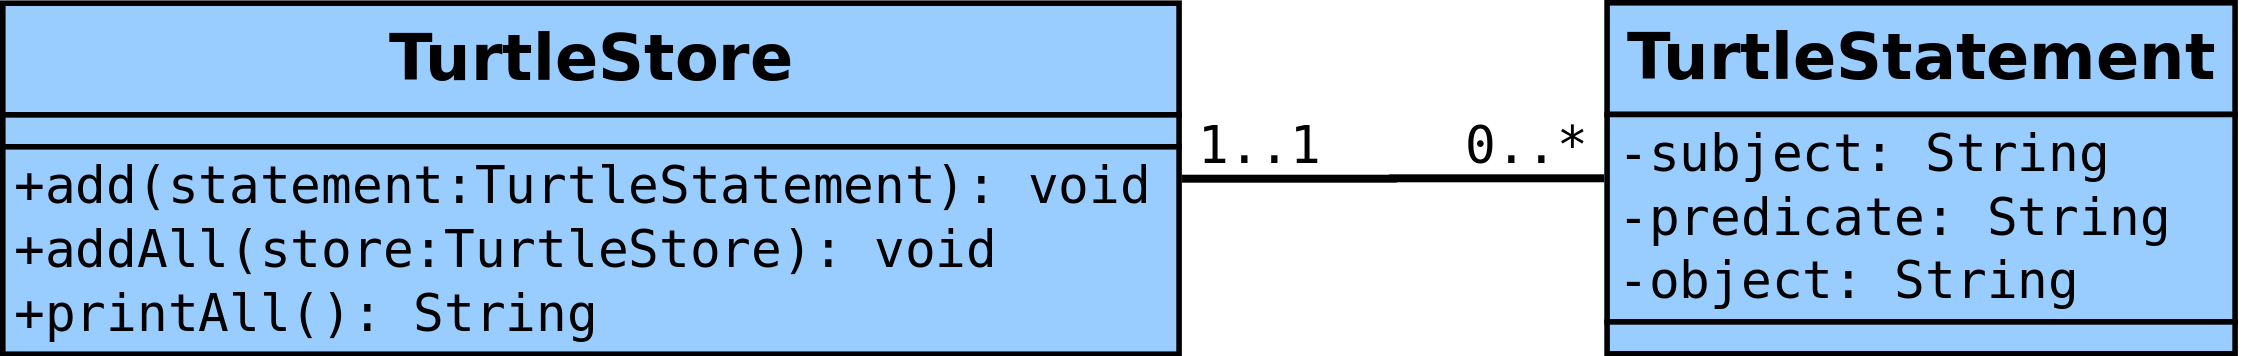
\includegraphics[width=.7\textwidth]{figures/diagrams/turtlestore.pdf}
\caption{Classes used for output in \emph{Turtle syntax}}
\label{fig:importer_turtlestore}
\end{figure}

Figure~\ref{fig:importer_turtlestore} shows the two classes \texttt{TurtleStatement} and \texttt{TurtleStore} that provide a data structure for output in \emph{Turtle syntax}. \texttt{TurtleStatement} represents a single \emph{RDF} statement in turtle syntax; \texttt{TurtleStore} encapsulates a set of \texttt{TurtleStatement} objects and provides a method for writing all statements to a file.

Section~\ref{sec:appendix_turtle_output} in the appendix shows a part of the output generated by \emph{Weather Importer} in \texttt{turtle} mode.

\section{Unit tests}
\label{sec:importer_tests}

\emph{Weather Importer} incorporates a set of \emph{JUnit}~\cite{junit} tests that covers reasoning in the \smarthomeweather ontology and the application itself. For testing correct reasoning, the \emph{Apache Jena} framework and the \emph{Pellet} reasoner are used.

The following test categories are implemented:
\begin{itemize}
  \item Tests for \emph{OWL} reasoning concerning single individuals of the ontology; e.g. an instance of \Egls{weather phenomenon} that has a \egls{has temperature value} property must be reasoned to be an instance of \egls{temperature}.
  \item Tests that involve reasoning for instances of several concepts; e.g. correct reasoning of \Egls{calm weather}.
  \item Tests for the import of weather data from \yrno.
  \item Tests for the output in \emph{Turtle syntax}.
\end{itemize}

% TODO mention untested parts
\begin{comment}
The following parts of the application are not covered by unit tests:

\begin{itemize}
  \item bla
  \item blubb
  \item foo
  \item bar
\end{itemize}
\end{comment}
